\chapter{kardSort}

\label{chap:kardSort}


kardSort is an online card sorting tool that was created by a single
developer as their master's thesis. It is a very intuitive and simple
tool that is easy and rewarding to use. That being said it does lack
in some features in comparison to its peers and might be a little too
simple for some users~\parencite{kardSort}.

\begin{figure}[tp] 
\centering
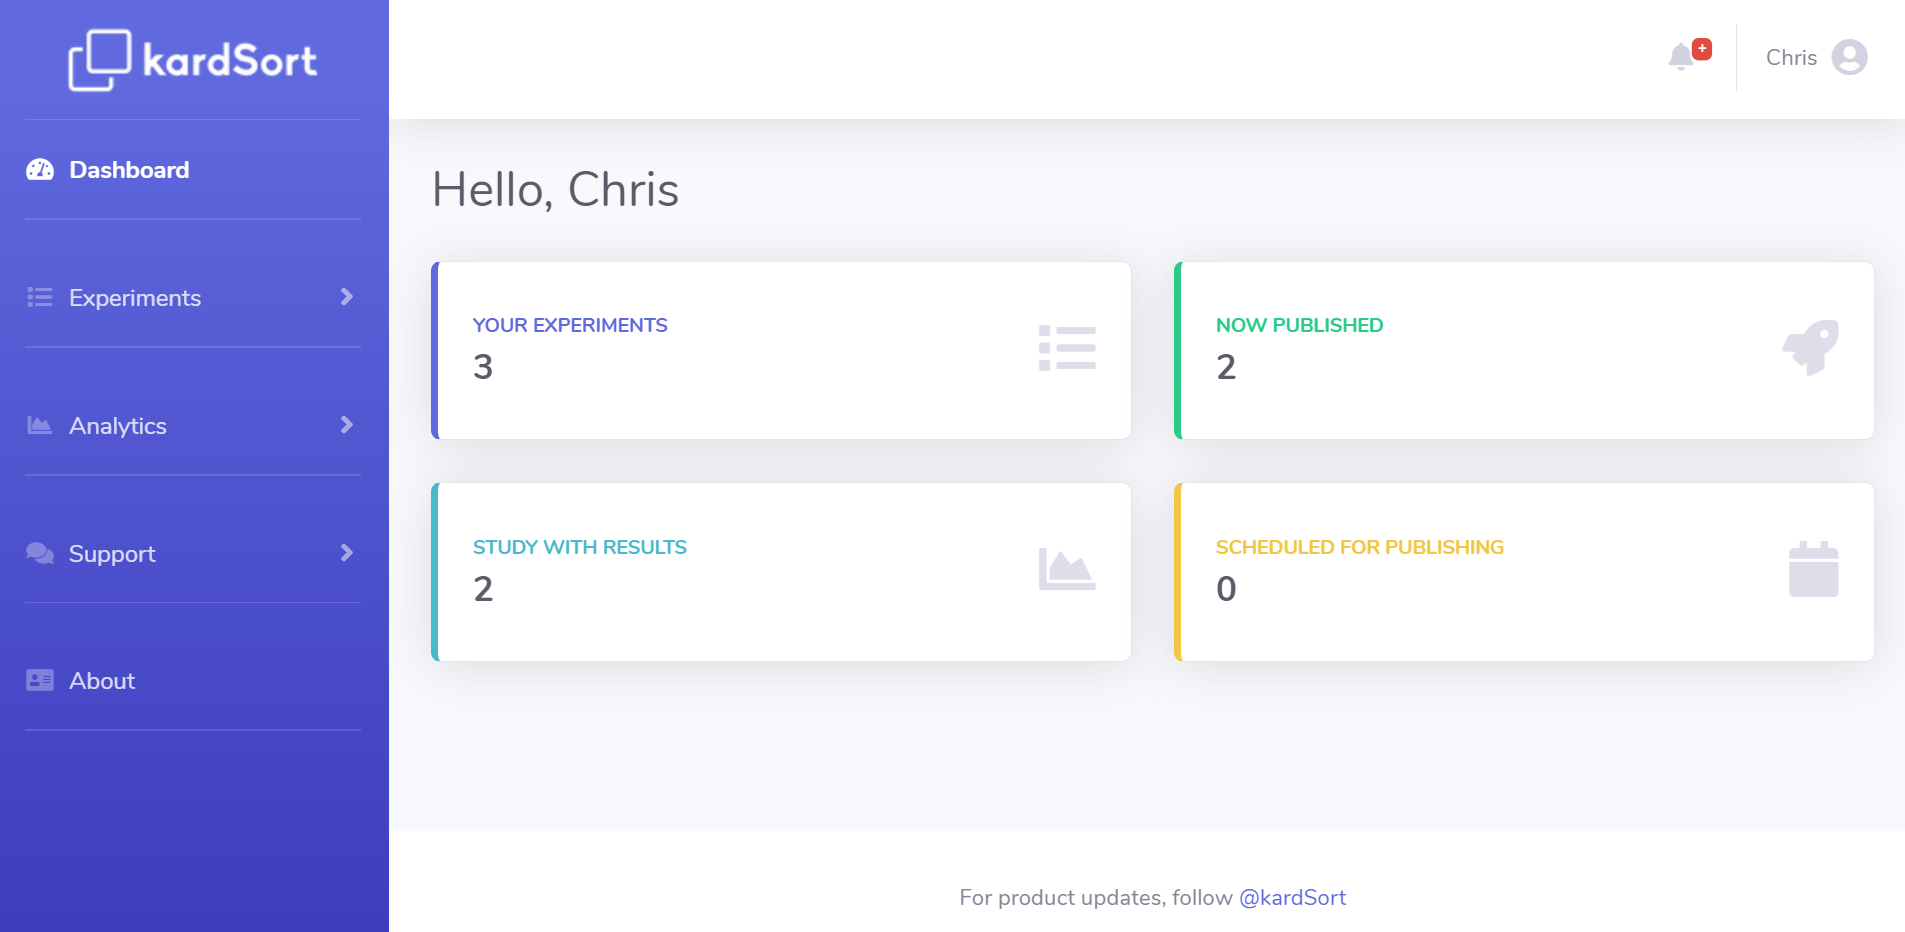
\includegraphics[keepaspectratio,width=\linewidth,height=\halfh]{images/kardsort-dashboard.png}
\caption[kardSort Application] { This is the base view in kardSort.
It shows you an overview of your experiments and in the side menu all
further actions can be performed.
\imgcredit{Screenshot was captured by Christopher Oser using
\textcite{kardSort} on Google Chrome 84.} }
\label{fig:kardSort1}
\end{figure}


\section{Business Model}
As to be expected from a master's thesis project the tool is fully 
free of charge. All features are accessible immediately and there are
no extra features hidden behind some paywall.

The only prerequisite for using the tool is to create an account,
either explicitly for the site or using an existing Google account.
The account make sure all the work within the tool is saved and can be
accessed again even after the session has been terminated. This also
enables access to the experiments, regardless of device or geo-
location. All experiments and data are saved in a cloud that is
provided by kardSort.

\section{Card Sorting}
The card sorting in kardSort is very straight forward. There are no 
special gimmicks or features that make it stand out from other tools.
They offer open, closed and hybrid card sorting. It is possible to
include a welcome message and instructions for every experiment.

A feature that is quite handy at times, is the possibility to include
a customizable questionnaire for an experiment. This questionnaire can
be made up of any number of single line text, multi line text,
check box or radio button questions and is displayed right before the
actual sorting.

In terms of limitations during card sorting, we were able to find two.
Firstly it is not possible to perform an experiment with more than 50
cards. This is a hard limit set during development that offers no
workaround by a user. If this is a deal-breaking limitation, it could
be possible to contact the developer about it and request more cards
per experiment, as the tool does have a feature request page.
Secondly it is quite exhausting working with more than five
categories, as the way the tool is defined, it adds new categories at
the very right of the previous categories. Therefore a lot of
horizontal scrolling is involved when browsing larger number of
categories.

A detailed summary of features can be viewed in
Table~\ref{tab:features-kardSort}.

\begin{figure}[tp] 
\centering
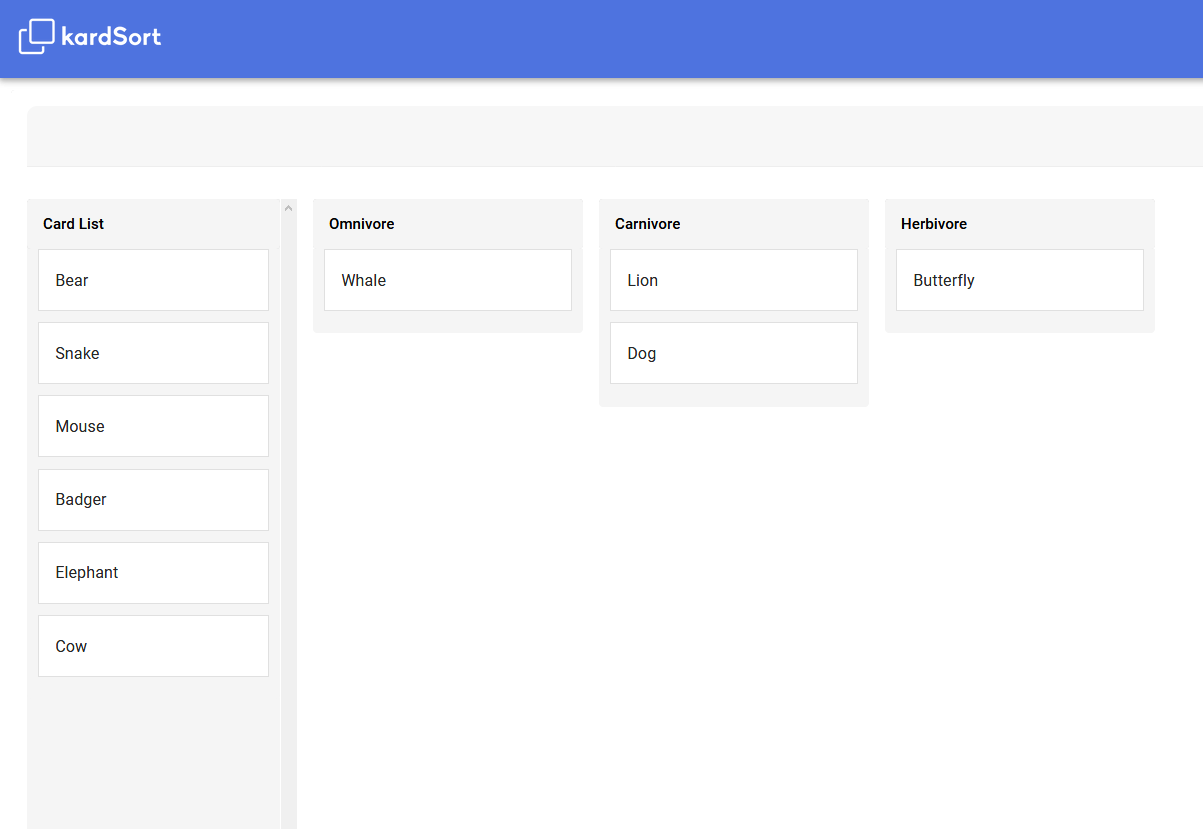
\includegraphics[keepaspectratio,width=\linewidth,height=\halfh]{images/kardsort-sorting.png}
\caption[kardSort Card Sorting] { This is a screenshot during the card
sorting process in kardSort.
\imgcredit{Screenshot was captured by Christopher Oser using
\textcite{kardSort} on Google Chrome 84.} }
\label{fig:kardSort2}
\end{figure}


\section{Analytics} This is the caveat of kardSort, the part where it
is truly lacking, because it does not offer any type of analytics for
its experiments. There is the  possibility of exporting all the
relevant data of an experiment to .csv files for manual analytics or
data preparation. 

Additionally it also offers to export experiment data in the required
format of two other card sorting analytics tools, namely Casolysis and
SynCaps. These two tools are both free of charge and provide good
analytics for card sorting experiments. Further information about them
can be found in the respective Chapters~\ref{chap:SynCaps} and
~\ref{chap:Casolysis} within this survey.

\begin{table}[tp]
\centering
\begin{tabularx}
{\linewidth}{|l|X|}
\hline \textbf{Feature/Characteristic} & \textbf{Availability in kardSort} \\ 
\hline Card Sorting & Open, closed and hybrid. \\ 
\hline Card Limit & 50 \\
\hline Participant Limit & None. \\
\hline Analytics & Only export for Casolysis and SynCaps. No in-tool
analytics \\ 
\hline Documentation & None, but tool explains itself very well. No 
documentation was needed during review. \\
\hline Business Model & Free. \\
\hline Import formats & None. All data needs to be entered by hand.\\ 
\hline Export formats & .csv for everything plus formats matching
Casolysis and SynCaps. \\ 
\hline Sub-Categories & No. \\ 
\hline Playback of user-sessions & No. \\ 
\hline Data preparation & Only by hand through export files. \\ 
\hline
\end{tabularx} 
\caption[Feature summary of kardSort] 
{ 
This table summarizes all the features and characteristics of kardSort
to provide an easy to read overview.
}
\label{tab:features-kardSort}
\end{table}


\section{Summary \& Ratings}
All in all kardSort provides a very good card sorting experience. 
Everything it does it does well. Apart from a card limit and some 
formatting with the categories there were no issues when reviewing 
the tool.

Of course it lacks greatly in comparison to other tools, since it 
does not provide any own analytics. Although it does provide you
with the option to do the analytics elsewhere. So this could be a
possible compromise for some users, making this nonetheless a viable
option when in search for a card sorting tool.

For a quick overview and to make it easier to compare to other tools
in this paper, we agreed on 4 ratings for the tool. The ratings can be
found in Table~\ref{tab:rating-kardSort} and range from 0-5.

\begin{table}[tp] 
\centering 
\begin{tabularx}{\linewidth}{|X|X|X|X|X|}
\hline
Simplicity & Documentation & Features & Business Model & Average \\ 
\hline 
5 & 1 & 1 & 5 & 3.0 \\ 
\hline 
\end{tabularx} 
\caption[Ratings for kardSort] {
Ratings for kardSort including the average rating.
} 
\label{tab:rating-kardSort}
\end{table}